\documentclass[12pt]{article}
\usepackage{geometry}                % See geometry.pdf to learn the layout options. There are lots.
\geometry{letterpaper}                   % ... or a4paper or a5paper or ... 
%\geometry{landscape}                % Activate for for rotated page geometry
\usepackage[parfill]{parskip}    % Activate to begin paragraphs with an empty line rather than an indent
\usepackage{daves,fancyhdr,natbib,graphicx,dcolumn,amsmath,lastpage,url}
\usepackage{amsmath,amssymb,epstopdf,longtable}
\DeclareGraphicsRule{.tif}{png}{.png}{`convert #1 `dirname #1`/`basename #1 .tif`.png}
\pagestyle{fancy}
\lhead{CE 3372 -- Water Systems Design}
\rhead{FALL 2015}
\lfoot{EXERCISE 3}
\cfoot{}
\rfoot{Page \thepage\ of \pageref{LastPage}}
\renewcommand\headrulewidth{0pt}

\begin{document}
\begin{center}
{\textbf{{ CE 3372 -- Water Systems Design} \\ {Exercise Set 3}}}
\end{center}

\section*{\small{Exercises}} 
Compute the discharge in each pipe and the pressure at each junction node for the 8-pipe system shown in Figure \ref{fig:primary-network}.   The water surface elevation in the storage tank is 315.0 ft.   Prepare your solution using EPA-NET.   Report your results in U.S. Customary units.   Identify the node with the lowest pressure in your solution.   Include a transmittal letter with the solution.   
\begin{figure}[h!] %  figure placement: here, top, bottom, or page
   \centering
   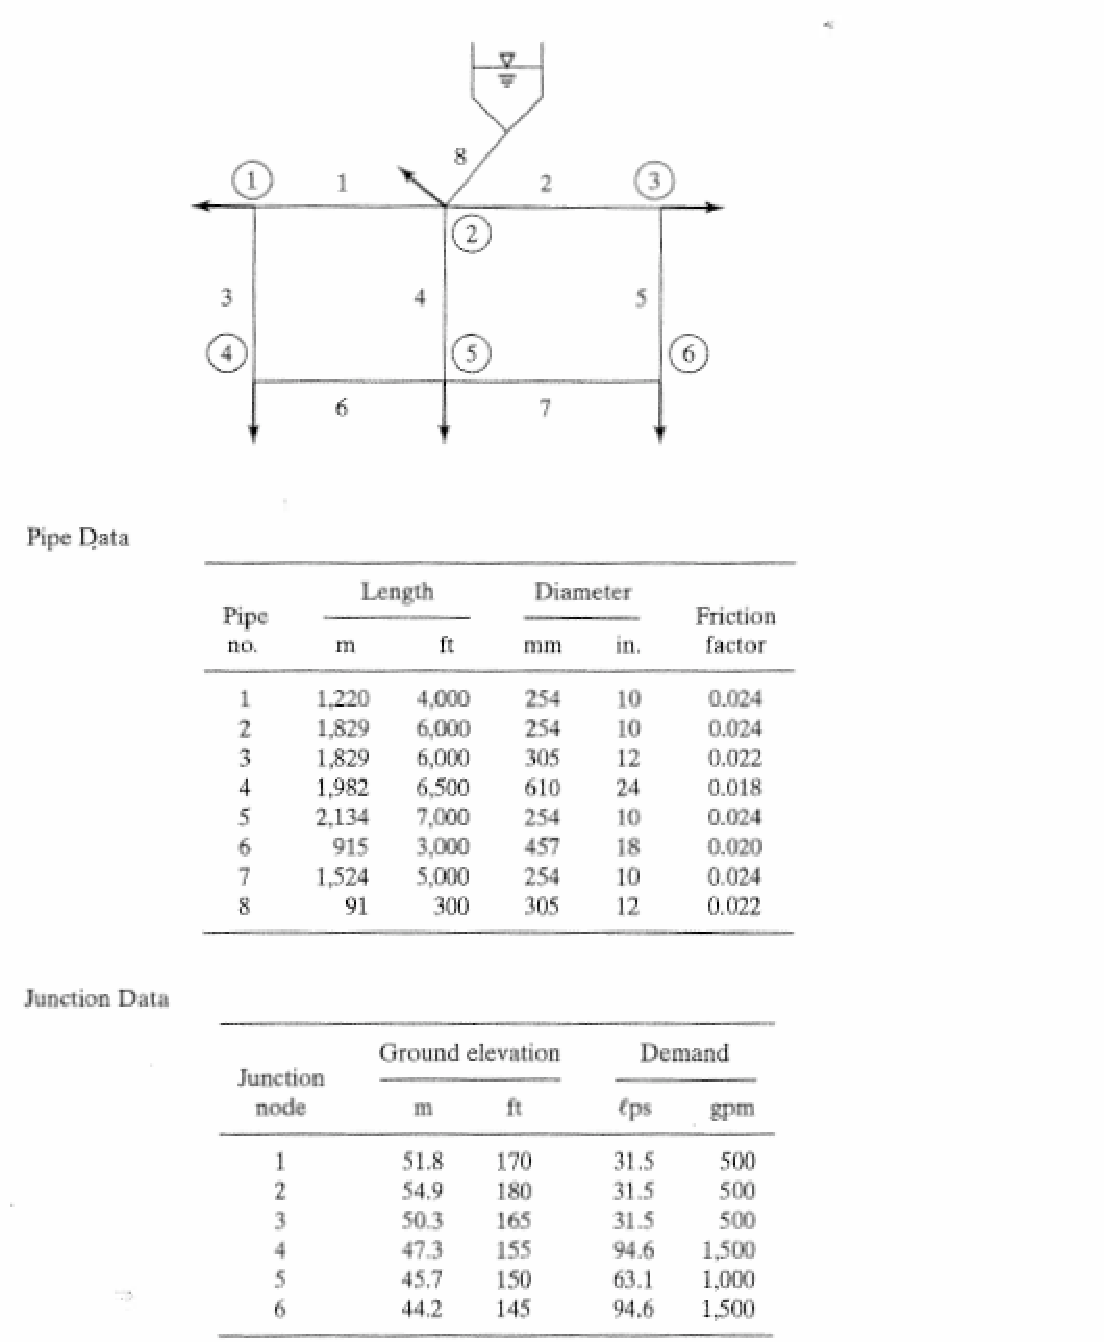
\includegraphics[height=5.2in]{primary-network.pdf} 
   \caption{Network for ES-3}
   \label{fig:primary-network}
\end{figure}





\end{document}  